\newpage

\section{Przygotowanie próbek do badań}

\subsection{Przyrząd pomiarowy, rysunek, opis}
\begin{figure}[H]
	\begin{center}
		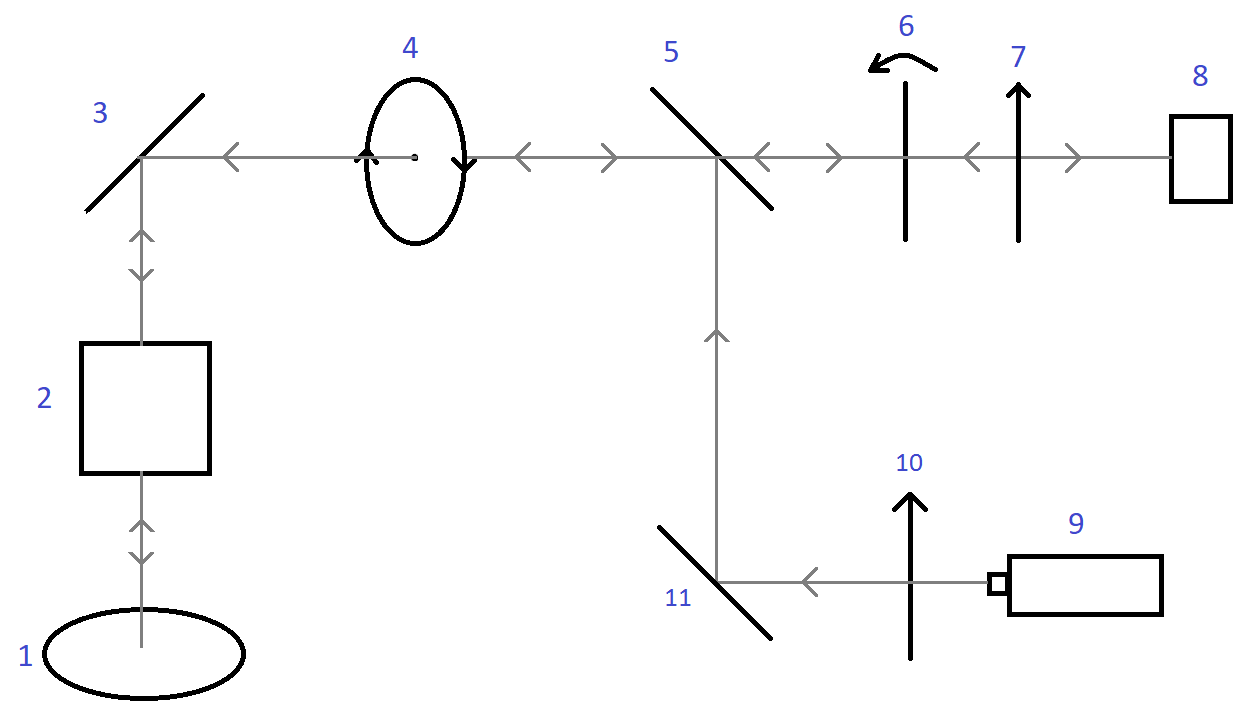
\includegraphics[width=1.0\linewidth]{Przygotowania/Uklad-pomiarowy.png}
		\caption{Schemat układu pomiarowego.}
	\end{center}
\end{figure}

\begin{itemize}
	\item 1 - Badana próbka, $\alpha$-$\mathbf{Ga_{2}S_{3}}$;
	\item 2 - Mikroskop;
	\item 3, 11 - Lustra;
	\item 4 - HWP\footnote{HWP z angielskiego ''Half-wave plate'' czyli  płytka półfalowa}, nazwa skrócona ''półfalówka'';
	\item 5 - Płytka pólprzepuszczająca;
	\item 6 - HWP 90$^{\circ}$, ustawiona tak że przekręca polaryzację o 90$^{\circ}$;
	\item 7, 10 - Polaryzatory;
	\item 8 - Detektor;
	\item 9 - Laser argonowy 514 nm;
\end{itemize}

Promieniowanie elektromagnetyczne o długości fali 514 nm, emitowane laserem argonowym (9), przechodzi przez pionowo ustawiony polaryzator (10). Chociaż fala elektromagnetyczna emitowana laserem już jest spolaryzowana, polaryzator (10) zapewnia dodatkową polaryzację. Dalej fala elektromagnetyczna odbija się od zwierciadła (11) i trafia na płytkę półprzepuszczającą (5). Zatem odbija się od tej płytki i przechodzi przez HWP (4), gdzie polaryzacja skręcona o określony kąt $\alpha$, po przejściu przez (4) polaryzacja fali elektromagnetycznej jest przekręcona o kąt 2$\alpha$. Dalej fala trafia na próbkę (1) przez (2). Rozproszona fala elektromagnetyczna na fononach trafia na zwierciadło (3), odbija się od tego zwierciadła i przechodzi prze ''półfalówkę'' (4). Teraz ''półfalówka'' względem światła rozproszonego ma skręcony kąt o $-\alpha$. Po przejściu przez (4) polaryzacja rozproszona fala elektromagnetycznej jest skręcona o -2$\alpha$. Dalej światło rozproszone trafia do ''półfalówki'' na stale przekręconej o 45$^\circ$ czyli fala, która przeszła przez (6) ma skręcony kąt polaryzacji o 90$^\circ$. Następnie po przejściu polaryzatora (7) fala elektromagnetyczna trafia na detektor z kamerą CCD. Polaryzator (7) jest po to aby zbierać światło rozproszone tylko o określonej polaryzacji.

Pomiar się odbywał w dwóch konfiguracjach:
\begin{itemize}
	\item VV - zbierane światło rozproszone w takim samym kierunku jak światło pobudzające\footnote{Światło emitowane laserem}. Bez HWP 90$^{\circ}$.
	\item VH - zbierane światło rozproszone w kierunku prostopadłym do światła pobudzającego. Z obecnością HWP 90$^{\circ}$.
\end{itemize} 

Charakterystyki pomiaru:
\begin{itemize}
	\item Czas pomiaru 30 sek;
	\item Środek detektora 1040 $cm^{-1}$;
	\item Moc lasera 10 \% z $\frac{3}{4}$ mocy maksymalnej;
	\item Polaryzacja lasera normalna;
	\item Długość fali 514 nm;
	\item Każdy pomiar skręcenie "półfalówki" co 5$^{\circ}$;
	\item Konfiguracja VV bez elementu (6) rys. 22. Konfiguracja VH z elementem (6).
	\item Oprogramowanie \textit{Wire} 4.2.
\end{itemize}

\textbf{\textcolor{red}{Zdjęcie i opis sprzętu pomiarowego, razem z oprogramowaniem}}.

Przy pomiarach powstawały niektóre trudności.

Płytka $\mathbf{GaP}$ ma wymiary 3mm x 2mm x 1mm. Kryształki które zostały utworzone na tej płytce były rzędu kilku mikrometrów. Poszukiwany kryształek do badań powinien przypominać sześciokąt, być osobnym kryształkiem i mieć płaską powierzchnię. Ta powierzchnia powinna być w miarę równoległa do podłoża.

Kryształki zostały utworzone na podłożu z $\mathbf{GaP}$. Piki na widmie ramanowskim pochodzące z galu nakładają się na niektóre piki pochodzące z $\mathbf{Ga_{2}S_{3}}$. To bardzo utrudnia analizę niektórych pików z $\mathbf{Ga_{2}S_{3}}$.

Kryształki zostały zdrapane papierem ściernym i przełożone na taśmę klejącą. Ale po kilku pomiarach ciepło które pochodzi od tego, że promieniowanie laserowe grzeje miejsce w które trafia. Taśma klejąca pod wpływem ciepła rozszerza się, co powoduje znaczącą rozkalibrację układu pomiarowego. 

Zostało podjęte ryzyko, że zdrapane kryształki należy przenieść na szklaną płytkę. Z tej płytki te kryształki można łatwo zdmuchnąć. To jest niebezpieczne dla tego, że cały pomiar może być robiony przez dwa dni po kilku godzin.

\subsection{Technologia wzrostu kryształków} 

$\mathbf{Ga_{2}S_{3}}$ posiada odmienną strukturę krystaliczną od $\mathbf{GaS}$ – żadna faza krystaliczna siarczku galu(III) nie wykazuje budowy warstwowej. W związku z tym otrzymywanie cienkich warstw $\mathbf{Ga_{2}S_{3}}$ nie jest możliwe w procesie eksfoliacji i wymaga zastosowania innych metod (np. CVD, MBE).

Warstwy $\mathbf{Ga_{2}S_{3}}$ były otrzymywane poprzez reakcję małych ilości par siarki z płytkami krystalicznego fosforku galu, które zostały wypolerowane z jednej strony.

W ampule kwarcowej umieszczono krystaliczną płytkę $\mathbf{GaP}$ \footnote{Płytka jest mała o wymiarach 5 x 3 x 1 mm.} oraz 1 mg krystalicznej siarki. Ampułę następnie zamknięto pod próżnią (<1 mbar) i wstawiono do pieca rurowego w taki sposób by płytka była w środku strefy grzejnej, a następnie rozpoczęto ogrzewanie ze wzrostem temperatury $1^{\circ}/min$ aż do osiągnięcia temperatury 600$C^{\circ}$
Reakcję prowadzono przez 4 dni, po których piec wyłączono i pozostawiono do naturalnego wystygnięcia.

Próbki były robione w ramach współpracy z wydziałem chemicznym w laboratorium wydziału chemicznego Politechniki Warszawskiej.

\begin{figure}[H]
	\begin{minipage}[h]{0.5\linewidth}
		\center{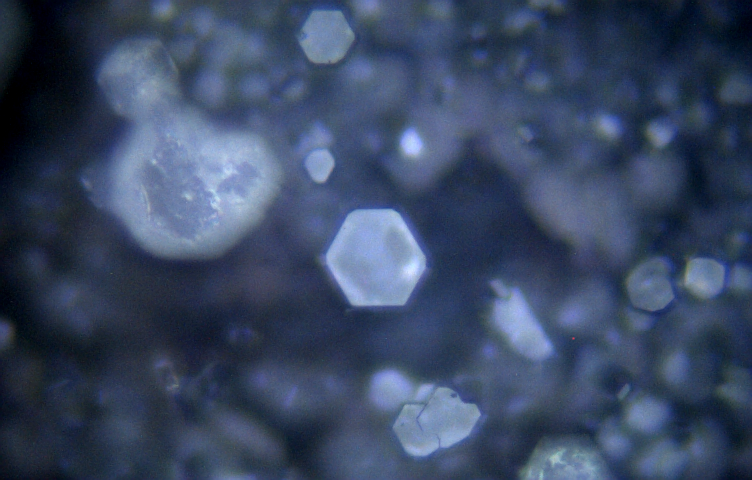
\includegraphics[width=0.8\linewidth]{Przygotowania/SLA39-50x-plytkiGa2S3.png}} \\ a) 
	\end{minipage}
	\hfill
	\begin{minipage}[h]{0.5\linewidth}
		\center{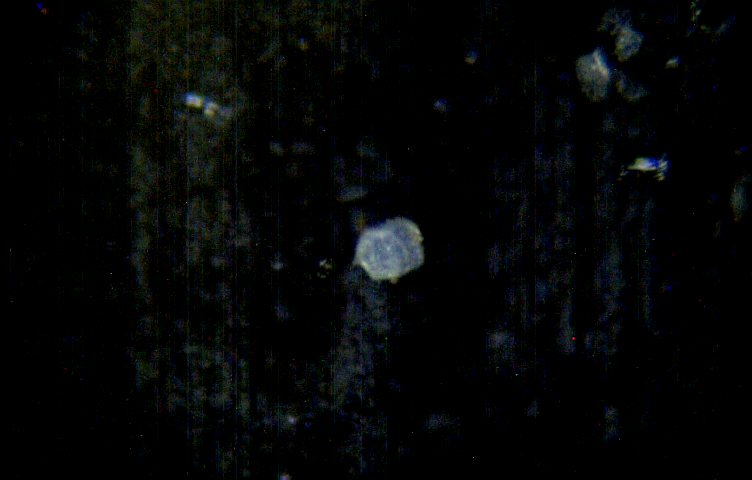
\includegraphics[width=0.8\linewidth]{Przygotowania/long50x.png}} \\b)
	\end{minipage}
	\caption{Kryształki badanego materiału $\mathbf{Ga_{2}S_{3}}$.}
\end{figure}

\begin{figure}[H]
	\begin{center}
		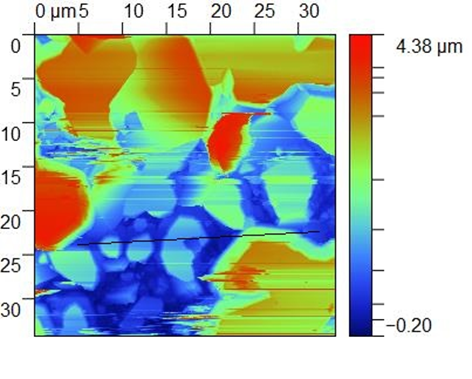
\includegraphics[width=0.65\linewidth]{Przygotowania/SEM.png}
		\caption{Skan typowej powierzchni uzyskanej w procesie syntezy.[36]}
	\end{center}
\end{figure}
























 